%!TEX root = ../../../2019main.tex
\vspace{10pt}
\subsubsection*{\bf Detector Charcterization}
\vspace{3pt}
\noindent {\sf [Spokesperson :\ Takahiro Yamamoto]}

\vspace{3pt}
\noindent {\sf \small ICRR, The Univ.\ of Tokyo, Hida, Gifu 506-1205}

\paragraph*{\bi Detector commissioning support}
The goal of detector characterization is providing the reliable data for gravitational waves searches.
In order to achieve this goal, we developed some data monitor tools such as SummaryPages shown in figure 1.
SummaryPage is the web-based data monitor system for supporting detector commissioning activities.
Commissioning activities are performed to achieve the stable operation of the interferometer and the target sensitivity. On the gravitational wave observation, more than 100,000 signals are acquired as the observational data.
SummaryPage helps us to monitor such a lot of signals efficiently.
In addition, since KAGRA joined the international observing network of gravitational waves, SummaryPage also served as an interface for LIGO, Virgo, and KAGRA to know each other's situation.

\paragraph*{\bi Observing data validation}
During the observing run in the end of March 2020, we also provided indicators of the data quality as another major role. 
These indicators are used to judge whether the data can be used for gravitational wave searches.  
For the joint gravitational wave search with LIGO and Virgo, we also established to share these data quality indicators. 

\begin{figure}
\begin{center}
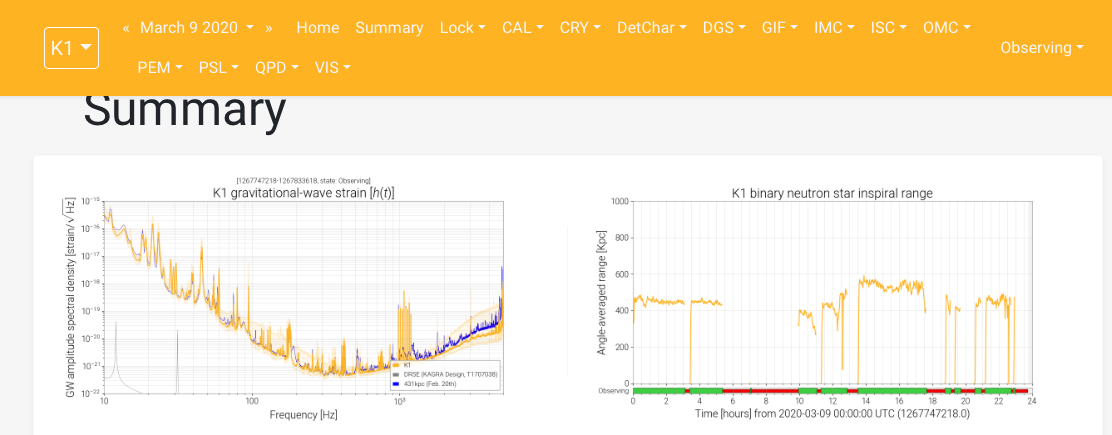
\includegraphics[width=0.48\textwidth]{astrodiv/gw/detc/png/det_summary.png}
\end{center}
\end{figure}
